
\subsection{Enemy Turn}
\label{Section_EnemyTurn}
After every player has finished playing their cards, move to the enemy turn. You need to \textbf{synchronise} the transition from player turn to enemy turn. 
If your group has trouble communicating this efficiently, you can turn your leftmost enemy \textbf{sideways as an indicator}. When everyone has their enemies turned sideways, it is time to proceed.
 
\begin{tcolorbox}[colframe=black, colback=white]
	Synchronising the transition is important since you may still receive help from an ally after you played all of your cards.
\end{tcolorbox}


\subsection*{Enemy Card}
\begin{figure}[ht]
	\begin{minipage}[t][5cm][t]{0.5\textwidth}
		Enemy cards consist of four parts:
		\begin{enumerate}
			\item \textbf{Name}	 - The name of the enemy
			\item \textbf{Passives} - Enemies can have passive effects too \textit{(See Enemy Keywords, page \pageref{Section_BoonsBanes})}
			\item \textbf{Life} - The life total is shown at the top right. When an enemy takes damage, place that many damage markers on that enemy. When the enemy has more damage markers than health, it dies
			\item \textbf{Actions} - enemies have one of two action patterns:\\
			\hspace*{1cm} \textbf{Dice} - Most enemies act according to the \hspace*{1cm} enemy die\\
			\hspace*{0.9cm} \textbf{ABC} - Some enemies repeat their \hspace*{1cm} actions in a pattern, indicated by letters
		\end{enumerate}
\begin{tcolorbox}[colframe=black, colback=white]
	 Track the actions of ABC enemies by placing a red enemy cube on their letter "A" at the start of combat. Move the cube down at the start of each turn.  When you reach the end, place the cube on "A" again.
\end{tcolorbox}		
		
	\end{minipage}	
	\begin{minipage}[t][10cm][t]{0.5\textwidth}
		\centering
		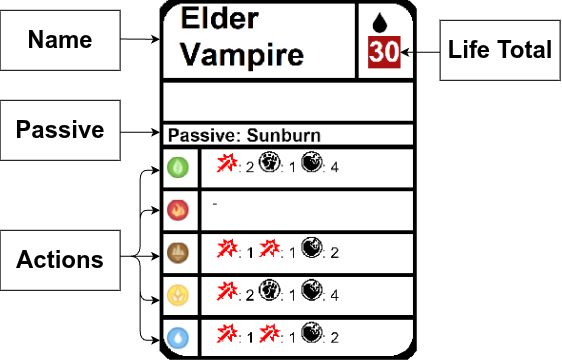
\includegraphics[width=0.9\linewidth, valign=t]{../ExplanationPics/MonsterCard.drawio.png}
		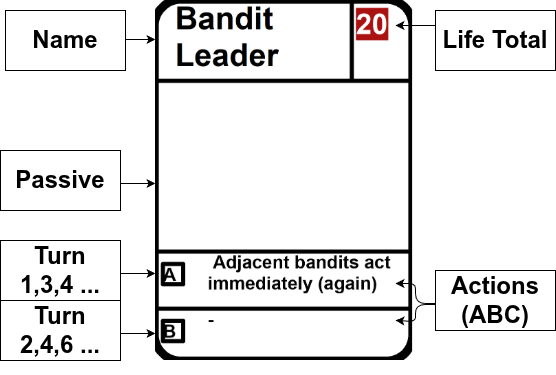
\includegraphics[width=0.9\linewidth, valign=t]{../ExplanationPics/MonsterCardABC.drawio.png}
	\end{minipage}
\end{figure}

\subsection*{Enemy actions}
Enemies always attack only the \textbf{player in front} of them. This means that all players can perform their enemy turn \textbf{simultaneously}. For each player, enemies act sequentially from left to right. 
To perform the enemy turn, look at the enemy die,  and have the enemy perform the corresponding action.
Repeat once for every enemy. All enemies use the same \textbf{global enemy die}.

\begin{figure}[ht]
	\begin{minipage}[t][6.5cm][t]{1\textwidth}
		\centering
		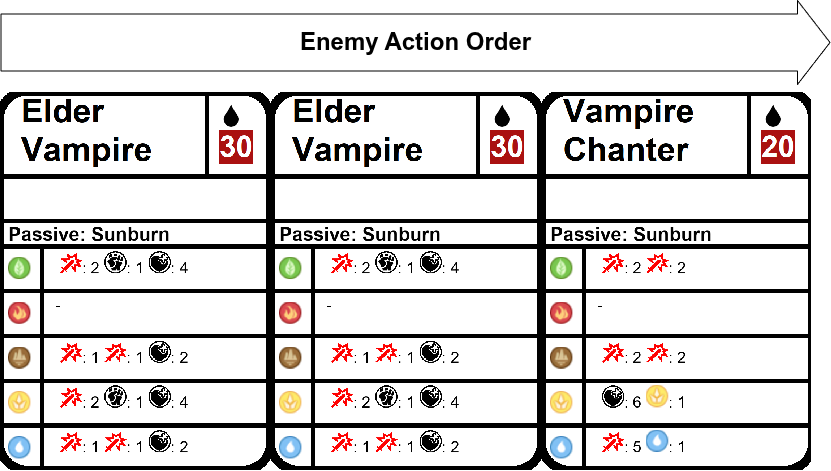
\includegraphics[width=0.9\linewidth, valign=t]{../ExplanationPics/MonsterTurn.drawio.png}
	\end{minipage}	
\end{figure}
\newpage
\textbf{Backlined} - If your life reaches 0, you are backlined. Your life cannot be raised above 0 for the \textbf{remainder of the fight}. You may still play a \textbf{single card per turn} while backlined.

\textbf{Enemy Focus} - Enemies will not finish a backlined player, and instead focus on the more dangerous active players. If your enemies are still acting, the rest of the enemies still perform their action. No remaining attack hits, but the enemies could still apply boons to themselves or each other. Afterwards, all of them rotate clockwise in the Cleanup step. When enemies rotate to you while backlined, immediately pass them to the next ally. You should have \textbf{no enemy in front of you while backlined}. Your allies still have to defeat these enemies to win.


